% \section{Evaluation}

% RQ1: completeness

% RQ2: correctness

% extendability

% usability 

\section{Validation of Semantics}\label{sec:validation}

Based on the kimulator, this section provides the approach to building confidence in our semantics and proposes several findings based on our validation results. \red{some fidings}

\begin{figure}
    \centering
    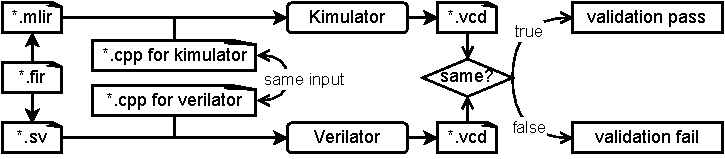
\includegraphics{fig/k-circt-co-simulation.drawio.pdf}
    \caption{Co-simulation against verilator for semantics validation.}
    \label{fig:co-simulation}
\end{figure}

Fig.~\ref{fig:co-simulation} offers an overview of our validation approach --- co-simulation against verilator. Given the same chisel, firrtl, or other hardware design source file using CIRCT, we can utilize the CIRCT project to compile them into generic mlir or verilog, which can be processed by kimulator and verilator, respectively. Then, we implement two Cpp source for the simulation of kimulator and verilator, and make sure they share the same input, such as the source files shown in Fig.\ref{fig:circt-example}. In the implementation, we also output the current state to a VCD file once after each evaluation. Thus, after the simulation, we can compare the VCD files proposed by kimulator and verilator, respectively. If they are logically identical, the validation for this test is passed; otherwise, the validation fails, and then we have to analyze and correct this error, since the error may be caused by several reasons, such as ambiguous documentation, error implementation of formal semantics, kimulator, verilator, or Cpp source file for simulation. 

The following presents two parts of the co-simulation experiments: (1) operation level validation: the test of each operation, and (2) hardware level validation: the test of combinations of operations to gain more confidence for real-world hardware.

% Mr.Zhao: 仿真时间上的对比。告诉我们是慢10倍（比如）。也是一个很重要的结论。 / 还有没有什么其他方面的内容可以做实验的。 / 比如内存消耗？

\smallskip
\textbf{Operation Level Validation}. This part presents test cases for each operation of core dialects in CIRCT and covers all the rewrite rules in the semantics, obtaining confidence for our constructed rules. Thus, we present \red{xx} tests for kimulator and verilator, respectively, since the existing test for CIRCT is for compiler test rather than a semantics test, thus is not complete to test each operation and rewrite rules in the semantics. For each test, we randomly generate \red{20} inputs in JSON and use the Cpp source file to make sure the input is sufficient and identical. The automatically generated inputs can be easily expanded, but we keep it at this magnitude in order to be able to do regression testing quickly. \red{Some operations require configuration for test input generation to cover all the rules in the semantics. For instance, operation \textit{comb.icmp} has xx comparison options. For each option, there is a rewrite rule to cover this. Thus, we configure the input test generator to make sure that for each option there are xx input.} \red{Additionally, most of the CIRCT operations cannot exist on their own. For example, the operations should be in the \textit{hw.module} operation for stimulation. And operations like \textit{sv.if} cannot be observed without a \textit{hw.output}. }

% \smallskip
% \textit{Test Input}.

\smallskip
\textit{Results}. \red{Our current implementation passes. xxx is incorrect. why? xxx is missing. why}

\smallskip
\textit{Inconsistent statement of MLIR syntax}. \red{provide a list in the appendix?}

\smallskip
\textit{Incomplete explanation of the operations}. \red{provide a list in the appendix? or write them in the project}

\smallskip
\textit{Other findings ....}
% 或许也可以讲一些K的问题？降低了我们的可用性？还是就不讲了


\smallskip
\textbf{Hardware Level Validation}. This part aims to test a combination of operations as part of real-world hardware, gaining confidence in the semantics completeness and usability for real-world hardware. \red{test from rocket?/verilator test? 5099 test files (https://github.com/verilator/verilator/tree/master/test\_regress/t)/part of rocket?/circt?} \red{we don't test xx, why}

\red{riscv-mini https://github.com/ucb-bar/riscv-mini/tree/main}


% \smallskip
% \textit{Test Input}.

\smallskip
\textit{Results}.
\begin{itemize}
    \item syntax errors in documentation
    \item syntax errors in implementation: twoState
\end{itemize}

\smallskip
\textit{finding1}. Some operation does not use in the compiled hardware.

\smallskip
\textit{Unstable version}.

\smallskip
\textit{inconsistency between CIRCT implementation and documentation}.

\smallskip
\textit{Other findings.... }.


% \subsection{Simulation Interface}
% 端口输入
% vcd对比统一对比结果
%% 为什么要自己构造？
%% 实验这一块核心语言语义是完整的。rocket。不一定要工程上很完美，但是要能跑。那可能就要比较好的benchmark。测试用例本身的完整性和覆盖度要说清楚。尽量把这个做了
%% 1. 如何选取和设置测试用例
%% 2. 如何使用这些测试用例进行测试
%% 3. 讨论测试结果
%% 最基本的测试是肯定要做的，application感觉可以根据需要进行加强
% verilog translates to mlir? using the test cases of verilator? rocket(感觉已经不是validation的问题了，而是规模化的问题)?

% sum-to-n: simulation validation, symbolic execution, program verification, translation validation
\section{Applications}

This section illustrates several applications of our semantics, demonstrating the potential role that semantics play in hardware design. Therefore, the following applications are illustrative cases rather than a comprehensive evaluation with scalability claims. We believe that each application can be further optimized to a standard tool, just like the kimulator we provided, since $\mathbb{K}$ is a language-agnostic framework and \cite{parkFormalVerificationTool2018,hathhornDefiningUndefinedness2015} also provided tools based on formal semantics in $\mathbb{K}$. We begin with the application derived from the extensibility of our semantics, followed by the applications proposed by the semantics' formal reasoning ability.

\subsection{Formalization of MLIR Dialects Semantics}

MLIR project~\cite{lattnerMLIRScalingCompiler2021} provides a parsimony builtin semantics, concepts, and interfaces to enable a high degree of freedom for crafting a high-performance compiler for customized representation. Thus, various fields leverage MLIR to provide their specific representation, e.g., machine learning, quantum computation, encryption algorithms, etc. This leads to at least 28 projects using MLIR, including CIRCT. And for each project, there are a lot of dialects to capture different abstractions. For example, the CIRCT project has 26 dialects in different abstraction levels to describe different hardware aspects. Thus, a convenient approach to constructing formal semantics for these dialects is necessary for moving toward a trustworthy MLIR.

We present dialect-agnostic semantics for MLIR in Section~\ref{sec:mlir-static-semantics}, allowing users to focus on developing dialect-specific semantics without concerning dialect-independent concepts, such as symbol tables and syntax differences between operations. Therefore, like what we did in Sections \ref{sec:circt-static-semantics} and \ref{sec:core-dialect-semantics}, it is straightforward to extend the program configuration for a specific domain and define the semantics for each operation in a uniform way. Furthermore, the semantics discussed in Section~\ref{sec:circt-static-semantics} provide program configuration enough for capturing the semantics of CIRCT, which means that it consists of enough state for real-world hardware simulation that proven by the \textit{hardware level validation}. This obviates the consideration of the state for other dialects of CIRCT. Not only that, the semantics in Section~\ref{sec:circt-static-semantics} also facilitate the development of \textit{preprocess} and \textit{stimulation} for dialect semantics in CIRCT by the predefined phases. 


\subsection{Hardware Verification}

Formal verification is important for hardware to provide rigorous guarantees for the correctness of the hardware. CC \& 

And while finding hard bugs is important, the big bonus is in a complementary verification strength to manage simulation overloads, to accelerate early maturing and to bail out slow programs.

We have found that the formal team is a great resource to pick up tasks where simulation teams aren’t yet ready to move over. Since formal doesn’t need to start with elaborate testbenches, they can often start finding bugs quickly and mature a block along the bug-finding cycle.

For example, % 乘法器


\subsection{Symbolic Simulation}

% 乘法器

\subsection{Translation Validation}

most imp

% 乘法器



% \section{Evaluation}
% \begin{itemize}
%     \item \textbf{RQ.1 (Extendable Capability)}: How can K-CIRCT be used to formalize the semantics of CIRCT dialects and what is the associated labor cost? %  Does the system's semantics accurately represent its intended meaning and behavior?
%     \item \textbf{RQ.2 (Reliability)}: To what extent can we trust the core semantics of CIRCT?
%     \item \textbf{RQ.3 (Applications)}: What are the applications of the formal semantics of CIRCT? (sum-to-n simulation validation, symbolic execution, program verification, translation validation) % 开关电路
% \end{itemize}